% !TEX root = ../main.tex

\begin{figure}[t]
    \centering
    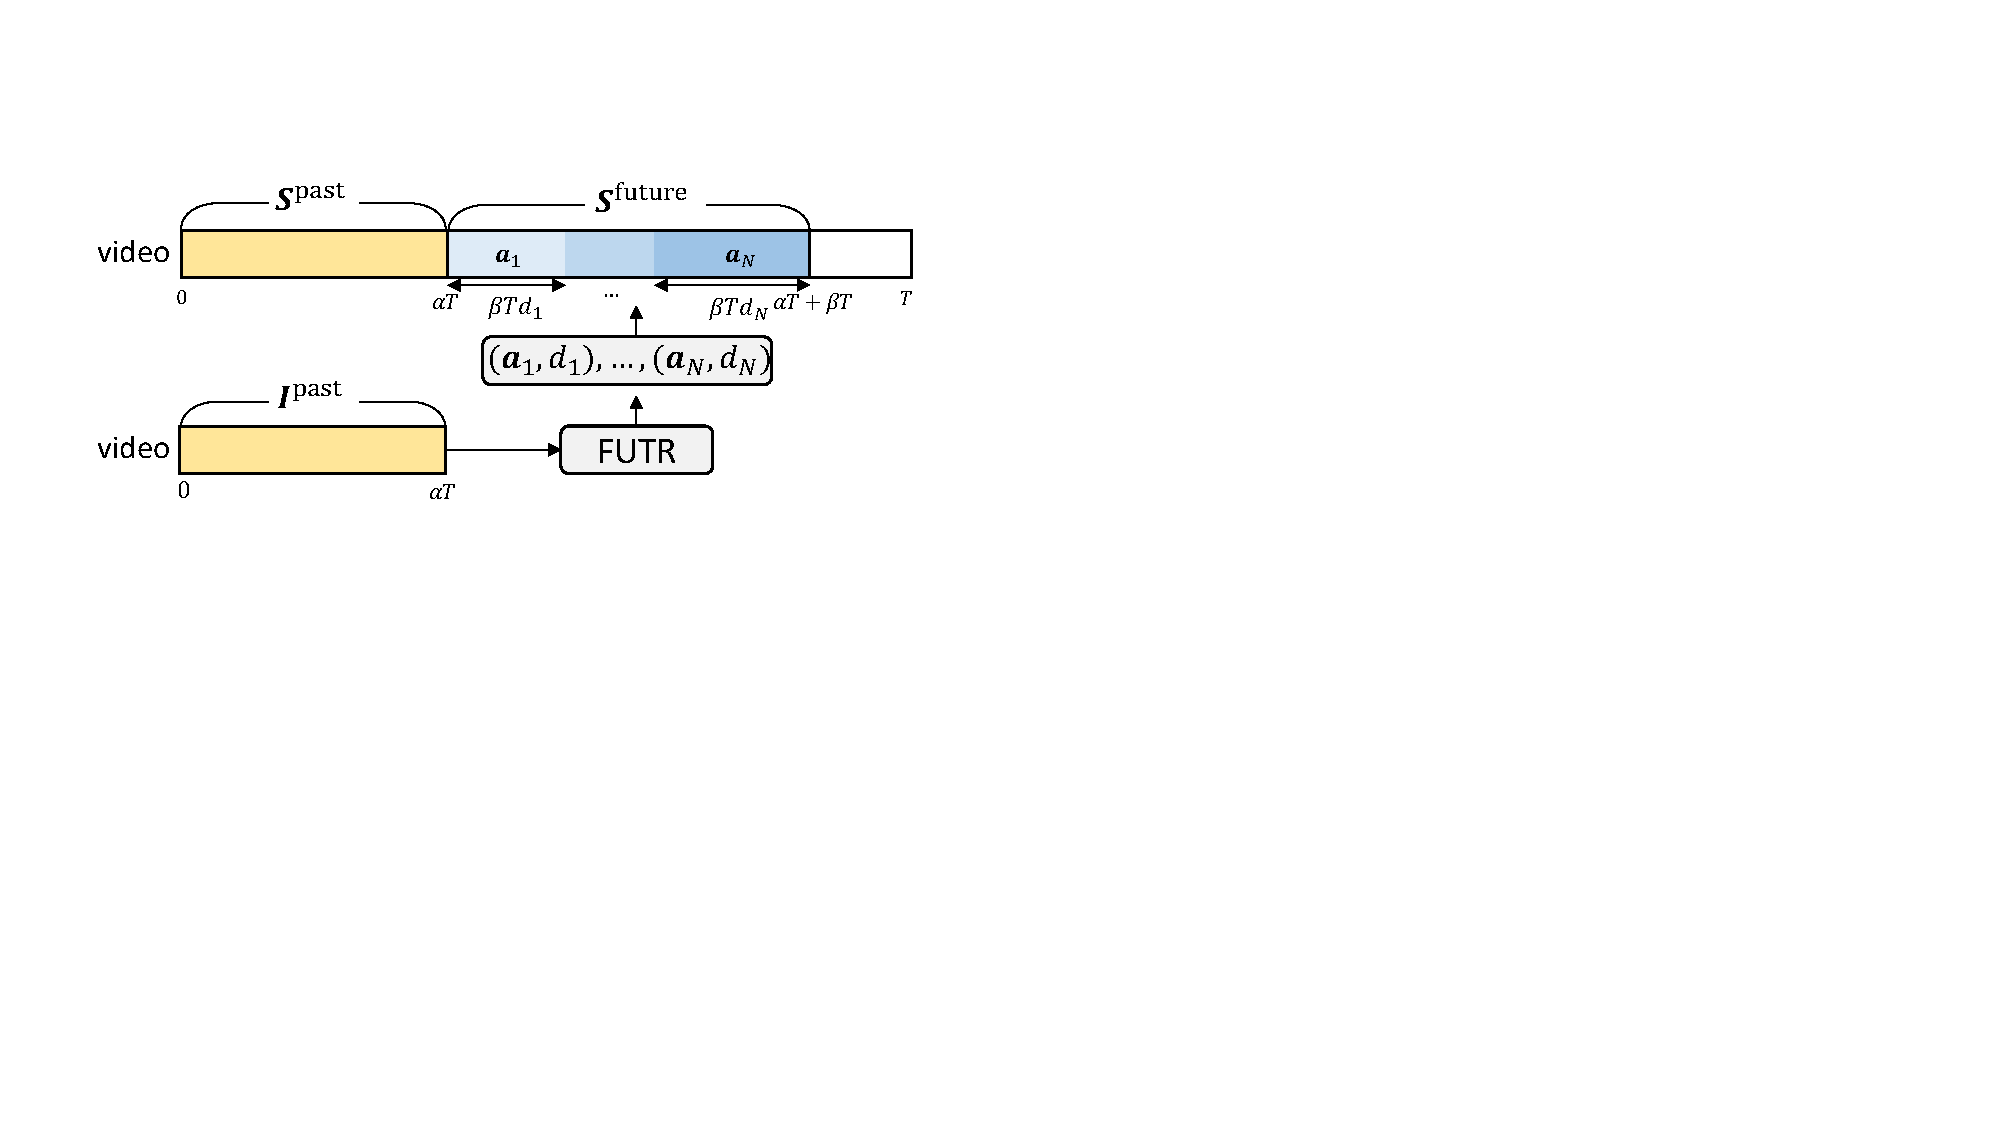
\includegraphics[width=0.98\linewidth]{Figures/pdf/task.pdf}
\caption{\textbf{Long-term action anticipation}.
The problem of long-term action anticipation aims to predict action labels of $\beta T$ future frames observing $\alpha T$ frames from a video, where $\alpha$ and $\beta$ indicate the observation and prediction ratio of the full video frames $T$, respectively. 
\ours anticipates action labels and durations of the $N$ action segments, where predicted action labels and duration are decoded into frame-level action labels for evaluation.}
\label{fig:task}
\vspace{-2mm}
\end{figure}
\section{Future Transformer~(\ours)}
In this section, we introduce a fully attention-based network, dubbed \ours, for long-term action anticipation.
The overall architecture consists of a transformer encoder and a decoder, as depicted in Fig.~\ref{fig:pipeline}.
Section~\ref{sec:4.1} explains the encoder, which segments action labels from the fine-grained visual features of past frames, Section~\ref{sec:4.2} describes the decoder, which predicts action labels and durations of future frames in parallel decoding, and then Section~\ref{sec:4.3} presents the training objective of the proposed method.

\subsection{Encoder}
\label{sec:4.1}
The encoder takes visual features as input and segments actions of past frames, learning distinctive feature representations via self-attention.
\\
\noindent
\textbf{Input embedding.}
As input to the encoder, we use visual features extracted from the input frames $\bm{I}^{\mathrm{past}}$, which are denoted by $\bm{F}^{\mathrm{past}} \in \mathbb{R}^{\alpha T \times C}$~\cite{farha2020long,sener2020temporal}.
We sample frames with a temporal stride of $\tau$, establishing $\bm{E} \in \mathbb{R}^{T^\mathrm{O} \times C}$ where $T^\mathrm{O}= \lfloor \frac{\alpha T}{\tau} \rfloor$ is the number of sampled frames.
The sampled frame features are fed to linear layer $\bm{W}^\mathrm{F} \in \mathbb{R}^{C \times D}$ followed by ReLU activation function to $\bm{E}$, creating input tokens $\bm{X}_0 \in \mathbb{R}^{T^\mathrm{O} \times D}$:
\begin{align}
    \bm{X}_0 = \mathrm{ReLU}(\bm{E} \bm{W}^\mathrm{F}).
    \label{eq:1}
\end{align}

\noindent
\textbf{Attention.}
The encoder consists of the $L^\mathrm{E}$ number of encoder layers.
Each encoder layer is composed of a multi-head self-attention (MHSA), layer normalization~(LN) and feed-forward networks~(FFN) with residual connection.
We define a multi-head attention~(MHA) based on the scaled dot-product attention~\cite{vaswani2017attention} with input variables $\bm{X}$ and $\bm{Y}$: 
\begin{align}
    \mathrm{MHA}(\bm{X},\bm{Y})&=[\bm{Z}_1,..,\bm{Z}_h]\bm{W}^\mathrm{O},
    \label{eq:2}
    \\
    \bm{Z}_i&=\mathrm{ATTN}_i(\bm{X},\bm{Y}),
    \label{eq:3}
    \\
    \mathrm{ATTN}_i(\bm{X},\bm{Y})&=\sigma(\frac{(\bm{X}\bm{W}^\mathrm{Q}_i)(\bm{Y}\bm{W}^\mathrm{K}_i)^\top}{\sqrt{D/h}})\bm{Y}\bm{W}^\mathrm{V}_i,
    \label{eq:4}
\end{align}
where $\bm{W}^\mathrm{Q}_i, \bm{W}^\mathrm{K}_i$ and $\bm{W}^\mathrm{V}_i  \in \mathbb{R}^{D \times D/h}$ are query, key, and value projection layer at $i^{\textrm{th}}$ head, respectively, $\bm{W}^\mathrm{O} \in \mathbb{R}^{D \times D}$ is an output projection layer, $h$ is the number of heads, and $\sigma$ indicates a softmax.
MHSA is based on MHA with the two same inputs:
\begin{align}
    \mathrm{MHSA}(\bm{X})&=\mathrm{MHA}(\bm{X},\bm{X}).
    \label{eq:5}
\end{align}
The output token $X_{l+1}$ is obtained from the $l^{\textrm{th}}$ encoder layer:
\begin{align}
    \bm{X}_{l+1} &= \mathrm{LN}(\mathrm{FFN}(\bm{X}_l') + \bm{X}_l'),
    \\
    \bm{X}_l' &= \mathrm{LN}(\mathrm{MHSA}(\bm{X}_l+\bm{P}) + \bm{X}_l),
\end{align}
where an absolute 1-D positional embeddings $\bm{P} \in \mathbb{R}^{T^\mathrm{O} \times D}$ is added to the input of the $l^\mathrm{th}$ layer $\bm{X}_l\in \mathbb{R}^{T^\mathrm{O} \times D}$ for each MHSA layer.

\begin{figure*}[t!]
    \centering
    
\includegraphics[width=\linewidth]{Figures/pdf/pipeline.pdf}
\caption{\textbf{Overall architecture of \ours.} The proposed method is composed of an encoder and a decoder; each classifies action labels of past frames~(action segmentation) and anticipates future action labels and corresponding durations~(action anticipation), respectively.
The encoder learns distinctive feature representation from past actions via self-attention, and the decoder learns long-term relations between past and future actions via self-attention and cross-attention.
For simplicity, we set the number of past frames $\alpha T$ as 5 and the number of object queries $M$ as 5 in this figure. Note that $(X_l)_i$ and $(Q_l)_i$ indicate $i^\mathrm{th}$ index of $X_l$ and $Q_l$, respectively. }
\label{fig:pipeline}
\vspace{-1mm}
\end{figure*}
\noindent
\textbf{Action segmentation.}
The final output of the last encoder layer $X_{L^{\mathrm{E}}}$ is utilized to generate action segmentation logits $\hat{\bm{S}}^{\mathrm{past}} \in \mathbb{R}^{T^{\mathrm{O}} \times K}$
by applying a fully-connected~(FC) layer $\bm{W}^{\mathrm{S}}\in\mathbb{R}^{D \times K}$ followed by a softmax:
\begin{align}
    \hat{\bm{S}}^\mathrm{past}&= \sigma(\bm{X}_{L^{\mathrm{E}}}\bm{W}^{\mathrm{S}}).
\end{align}


%%%%%%%%%%%%%%%%%%%%%%%%%%%%%%%%%%%%%%%%%%%%%%%%%%%%%
%Decoder
\subsection{Decoder}
\label{sec:4.2}
The decoder takes learnable tokens as input, referred to as \textit{action queries}, and anticipates future action labels and corresponding durations in parallel, learning long-term relations between past and future actions via self-attention and cross-attention. 
\noindent
\\
\textbf{Action query.}
Action queries are embedded with $M$ learnable tokens $\bm{Q} \in \mathbb{R}^{M \times D}$.
The temporal orders of the queries are fixed to be equivalent to that of the future actions, \ie, the $i^{\textrm{th}}$ query corresponds to the $i^{\textrm{th}}$ future action.
We demonstrate that fixing temporal orders of the queries is effective for long-term action anticipation~(\Sec{5.4}).

\noindent
\textbf{Attention.}
The decoder consists of $L^\mathrm{D}$ number of decoder layers. Each decoder layer is composed of an MHSA, a multi-head cross-attention~(MHCA), LN, and FFN. 
The output query $\bm{Q}_{l+1}$ is obtained from the $l^{\textrm{th}}$ decoder layer:
\vspace{-1mm}
\begin{align}
    {\bm{Q}}_{l+1} &= \mathrm{LN}(\mathrm{FFN}({\bm{Q}}_l'') + {\bm{Q}}_l''),
    \\
    {\bm{Q}}_l'' &= \mathrm{LN}(\mathrm{MHA}(\bm{Q}_l'+\bm{Q},\bm{X}_{L^\mathrm{E}}+\bm{P}) + {\bm{Q}}_l'),
    \\
    {\bm{Q}}_l' &= \mathrm{LN}(\mathrm{MHSA}(\bm{Q}_{l}+\bm{Q})+{\bm{Q}}_l),
    \\
    \bm{Q}_0 &= [0, \dots, 0]^\top \in \mathbb{R}^{M\times D},
\end{align}
where $\bm{X}_{L^\mathrm{E}}$ is the final output of the encoder.
Note that action query $Q$ is added to the input of the $l^{\mathrm{th}}$ layer $Q_l\in\mathbb{R}^{M\times D}$ for each MHSA layer.
We initialize the input of the first decoder layer $Q_0$ with zero vectors.
%%%%%%%%%%%%%%%%%%%%%%%%%%%%%%%%%%%%%%%%%%%%%%%%%%%%%
\begin{table*}[t!]
\vspace{2mm}
\begin{center}
\scalebox{0.95}{
\begin{tabular}{C{1.7cm}C{1.7cm}wl{3cm}C{0.9cm}C{0.9cm}C{0.9cm}C{0.9cm}C{0.9cm}C{0.9cm}C{0.9cm}C{0.9cm}}
\toprule
\multirow{2}*[-0.5ex]{dataset} & \multirow{2}*[-0.5ex]{input type} & \multirow{2}*[-0.5ex]{methods} &\multicolumn{4}{c}{$\beta~(\alpha=0.2)$} & \multicolumn{4}{c}{$\beta~(\alpha=0.3)$}\\
\cmidrule( r){4-7}
\cmidrule( l){8-11}
&&&0.1 & 0.2 & 0.3 & 0.5& 0.1 & 0.2 & 0.3 & 0.5 \\
\cmidrule{1-11}
\multirow{8}*[-0.5ex]{Breakfast} &\multirow{4}*[-0.5ex]{label}& RNN~\cite{abu2018will}  &18.11 & 17.20 & 15.94 & 15.81 &21.64 & 20.02 & 19.73 & 19.21 \\
&&CNN~\cite{abu2018will}        &17.90 & 16.35 & 15.37 & 14.54 &22.44 & 20.12 & 19.69 & 18.76 \\
&&UAAA~(mode)~\cite{abu2019uncertainty} & 16.71 & 15.40 & 14.47 & 14.20 & 20.73 & 18.27 & 18.42 & 16.86 \\
&&Time-Cond.~\cite{ke2019time}  &18.41 & 17.21 & 16.42 & 15.84 &22.75 & 20.44 & 19.64 & 19.75 \\
\cmidrule{3-11}
&\multirow{4}*[-0.5ex]{features}&CNN~\cite{abu2018will} &12.78 & 11.62 & 11.21 & 10.27 & 17.72 & 16.87 & 15.48 & 14.09 \\
&&Temporal Agg.~\cite{sener2020temporal} &24.20 & 21.10 & 20.00 & 18.10 & \underline{30.40} & 26.30 & 23.80 & 21.20 \\
&&Cycle Cons.~\cite{farha2020long}    &\underline{25.88} & \underline{23.42} & \underline{22.42} &\underline{21.54} & 29.66 & \underline{27.37} & \underline{25.58} & \underline{25.20} \\ 
&&\ccol\textbf{\ours~(ours)}     &\ccol \textbf{27.70} & \ccol \textbf{24.55} & \ccol \textbf{22.83} & \ccol \textbf{22.04} &\ccol \textbf{32.27} & \ccol \textbf{29.88} &\ccol \textbf{27.49} &\ccol \textbf{25.87}\\
\cmidrule{1-11}
\multirow{7}*[-0.5ex]{50 Salads}&\multirow{4}*[-0.5ex]{label} & RNN~\cite{abu2018will}  &30.06 & 25.43 & 18.74 & 13.49 & 30.77 & 17.19 & 14.79 & 09.77 \\
&&CNN~\cite{abu2018will}        & 21.24 & 19.03 & 15.98 & 09.87 & 29.14 & 20.14 & 17.46 & 10.86 \\
&&UAAA~(mode)~\cite{abu2019uncertainty} & 24.86 & 22.37 & 19.88 & 12.82 & 29.10 & 20.50 & 15.28 & 12.31\\
&&Time-Cond.~\cite{ke2019time}  &32.51 & 27.61 & 21.26 & \underline{15.99} & \underline{35.12} & \textbf{27.05} & \underline{22.05} & \underline{15.59} \\
\cmidrule{3-11}
&\multirow{3}*[-0.5ex]{features}&Temporal Agg.~\cite{sener2020temporal} &25.50 & 19.90 & 18.20 & 15.10 & 30.60 & 22.50 & 19.10 & 11.20 \\
&&Cycle Cons.~\cite{farha2020long}    &\underline{34.76} & \textbf{28.41} & \underline{21.82} & 15.25 & 34.39 & 23.70 & 18.95 & \textbf{15.89} \\ 
&&\ccol\textbf{\ours~(ours)}     &\ccol \textbf{39.55} & \ccol \underline{27.54} & \ccol \textbf{23.31} & \ccol \textbf{17.77} &\ccol \textbf{35.15} & \ccol \underline{24.86} &\ccol \textbf{24.22} &\ccol 15.26\\
\bottomrule
\end{tabular}
}
\end{center}
\vspace{-4mm}
\caption{\textbf{Comparison with the state of the art.} Our models set a new state of the art on Breakfast, and 50 Salads. The numbers in bold-faced and in underline indicates the highest and the second highest accuracy, respectively.}
\label{tab:sota}
\vspace{-2mm}
\end{table*}

% C{0.75cm}C{1cm}C{0.9cm}C{0.9cm}C{0.9cm}C{0.9cm}C{0.9cm}
% cclcccccccc
% C{2cm}C{2cm}L{3cm}C{0.9cm}C{0.9cm}C{0.9cm}C{0.9cm}C{0.9cm}C{0.9cm}C{0.9cm}C{0.9cm}
\noindent
\textbf{Action anticipation.} 
The final output of the last decoder layer $Q_{L^{\mathrm{D}}}$ is utilized to generate future actions logits $\hat{\bm{A}} \in \mathbb{R}^{M \times (K+1)}$ by appling a FC layer $\bm{W}^{\mathrm{A}}\in \mathbb{R}^{D \times K+1}$ followed by a softmax and duration vectors $\hat{\bm{d}} \in \mathbb{R}^{M}$ by applying a FC layer $\bm{W}^\mathrm{D}\in \mathbb{R}^{D}$:

\begin{align}
    \hat{\bm{A}}&=\sigma(\bm{Q}_{L^{\mathrm{D}}}\bm{W}^\mathrm{A}),
    \\
    \hat{\bm{d}}&=\bm{Q}_{L^{\mathrm{D}}}\bm{W}^\mathrm{D}.
\end{align}
Note that if none of the future actions are predicted, we let the queries predict a dummy class, `\textit{NONE},' resulting in a total of $K+1$ classes.

\subsection{Training objective}
\label{sec:4.3}
\noindent \textbf{Action segmentation loss.}
We apply action segmentation loss to learn distinctive feature representations of past actions in the encoder as an auxiliary loss.
The action segmentation loss $\mathcal{L}^{\mathrm{seg}}$ is defined with the cross-entropy loss between target actions $\bm{S}^{\mathrm{past}}$ and logits $\hat{\bm{S}}^{\mathrm{past}}$:
\begin{align}
    \mathcal{L}^{\mathrm{seg}} &= -\sum^{T^\mathrm{O}}_{i=1}\sum^{K}_{j=1} \bm{S}^{\mathrm{past}}_{i,j}\log\hat{\bm{S}}^{\mathrm{past}}_{i,j}.
\end{align}
\noindent 
\textbf{Action anticipation losses.}
The $M$ number of action queries are matched to the $N$ number of ground-truth actions to apply action anticipation losses.
% If none of the future actions is predicted, we let the queries predict a dummy class, `\textit{NONE}.'
Action anticipation loss $\mathcal{L}^{\mathrm{action}}$ is defined with the cross-entropy between target actions $\bm{A}$ and logits $\hat{\bm{A}}$, and duration regression loss $\mathcal{L}^{\mathrm{duration}}$ is defined with L2 loss between target durations $\bm{d}$ and the predicted durations $\hat{\bm{d}}$ :
\begin{align}
    \mathcal{L}^{\mathrm{action}} &= - \sum^{M}_{i=1} \sum^{K+1}_{j=1} \mathbbm{1}_{i \leq \delta} \bm{A}_{i,j}\log(\hat{\bm{A}}_{i,j}),
    \\
    \mathcal{L}^{\mathrm{duration}} &= \sum^M_{i=1} \mathbbm{1}_{\mathrm{argmax}(\hat{\bm{A}}_i) \neq \mathrm{\textit{NONE}}} ( \bm{d}_{i} - \hat{\bm{d}}_i )^2,
\end{align}
where $\delta$ is the position of the first query that predicts \textit{NONE} and $\mathbbm{1}_{i \leq \delta}$ is an indicator function that sets to one where the query position $i$ is less than or equal to $\delta$.
$\mathbbm{1}_{\mathrm{argmax}(\hat{\bm{A}}_i) \neq \mathrm{\textit{NONE}}}$ is also an indicator function that sets to one where the predicted action of the $i^{\mathrm{th}}$ query is not \textit{NONE}.
Note that we apply gaussian normalization to the predicted duration to make summation of the whole durations as 1 following the previous work~\cite{abu2018will,farha2020long}.

\noindent
\textbf{Final loss.} The overall training objective $\mathcal{L}^{\mathrm{total}}$ is the sum of action segmentation loss, action anticipation loss, and duration regression loss:
% The final loss $\mathcal{L}^{\mathrm{total}}$ is defined by
\begin{align}
    \mathcal{L}^{\mathrm{total}} &=\mathcal{L}^{\mathrm{seg}}+ \mathcal{L}^{\mathrm{action}} + \mathcal{L}^{\mathrm{duration}}.
\end{align}
